% 2nd-iso-texse.tex
% see https://tex.stackexchange.com/a/482379/23098

\documentclass[tikz, margin=3mm]{standalone}
\usetikzlibrary{chains, positioning, shapes.geometric, fit}
\makeatletter
\tikzset{suspend join/.code={\def\tikz@after@path{}}}
\makeatother

\begin{document}
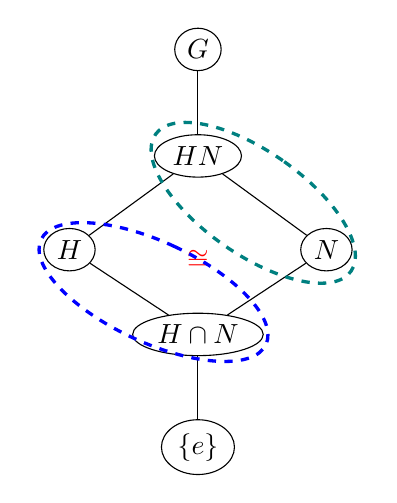
\begin{tikzpicture}[node distance = 8mm and 10 mm, 
	start chain = going below, 
    N/.style = {ellipse, draw, inner sep=2pt, on chain, join=by -}]
  \node (g)       [N] {$G$};
  \node (hn)      [N] {$HN$};
  \node (h)       [N, below left = of hn] {$H$};
  \node (hcapn)   [N, below = of h -| hn] {$H \cap N$};
  \node (e)       [N] {$\{ e \}$};
  %
  \node (n)       [N,suspend join, below right = of hn] {$N$};
  \node [below = of hn, red] {$\cong$};
  \draw (hn) -- (n)   (n) -- (hcapn);

  \node[very thick, teal, rotate = 55, ellipse, draw, dashed, inner xsep = -8mm, inner ysep = 2mm, fit=(hn)(n)] {};
  \node[very thick, blue, rotate = 65, ellipse, draw, dashed, inner xsep = -9.5mm, inner ysep = 3mm, fit=(hcapn)(h)] {};
\end{tikzpicture}
\end{document}
